\documentclass{article}
\usepackage[a4paper,left=0.5cm,right=0.5cm,top=0.5cm,bottom=0.5cm,bindingoffset=5mm]{geometry}
\usepackage{polyglossia}				%Sprache
\usepackage{amsmath}					%Matheumgebung
\usepackage{amsopn}					%Matheoperatoren
\usepackage{amssymb}					%Mathesymbole
\usepackage{amsthm}					%Mathetheorem
\usepackage{bbm}
\usepackage[autostyle=true,
			 german=quotes]
			 {csquotes}					%Anführungszeichen
\usepackage{mathdots}					%Punkte
\usepackage{mathtools}					%Bugfix ams
\usepackage{microtype}					%Makrotypographie
\usepackage{physics}					%Physiksymbole
\usepackage{pdfpages}
\usepackage{relsize}						%Größenangaben
\usepackage{scrhack}					%Verbesserung Pakete
\usepackage[separate-uncertainty,
			per-mode=symbol]
			{siunitx}					%Einheiten
\usepackage{textcomp}
\usepackage{tikz}						%Zeichnen
\usepackage{upgreek}					%Griechische Buchstaben
\usepackage{xltxtra}						%fontec
\setmainlanguage{english}
\setcounter{tocdepth}{1}
\setcounter{secnumdepth}{1}
\usepackage{enumitem}
\usepackage[bookmarksopenlevel=section,
			linkcolor=blue,
			colorlinks=true,
			urlcolor=blue,
			citecolor=blue]
			{hyperref}		%Verweise, muss am Ende stehen	
\usepackage{listings}
\usepackage{subfigure}
\usepackage{subfigure}
\begin{document}

\begin{figure}
\centering
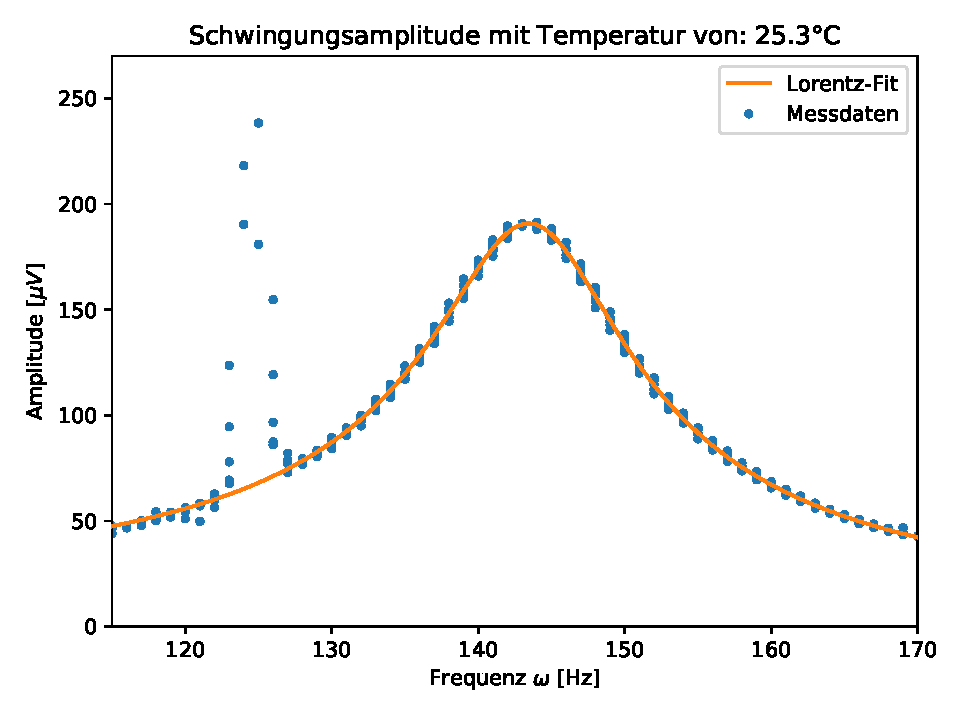
\includegraphics[width=0.5\textwidth]{Resonanz140_temp1.pdf}
\end{figure}
\begin{figure}
\centering
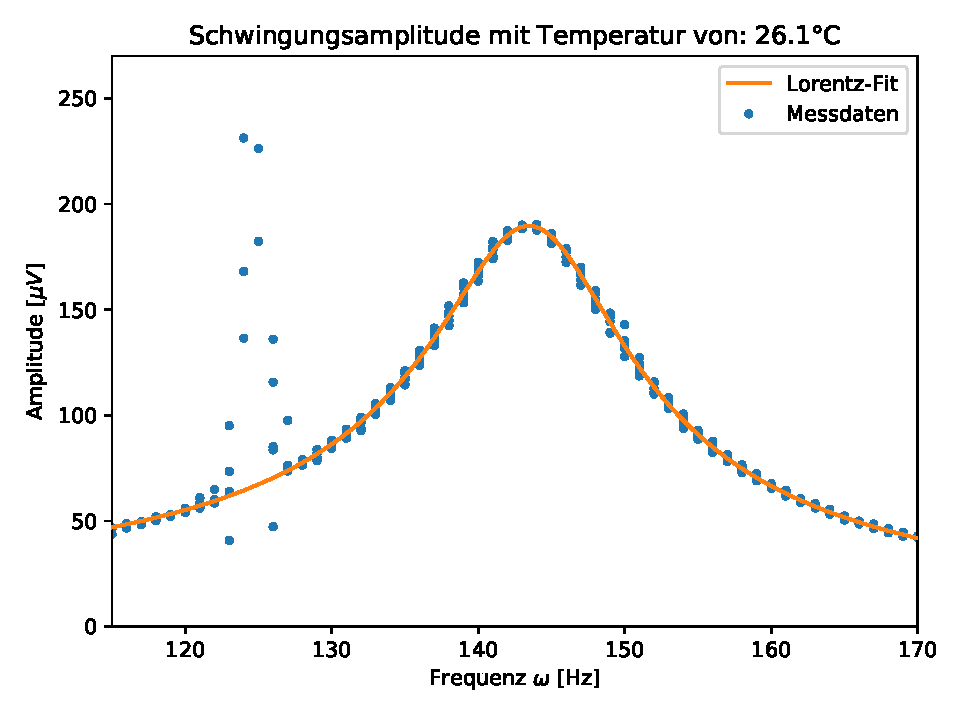
\includegraphics[width=0.5\textwidth]{Resonanz140_temp2.pdf}
\end{figure}
\begin{figure}
\centering
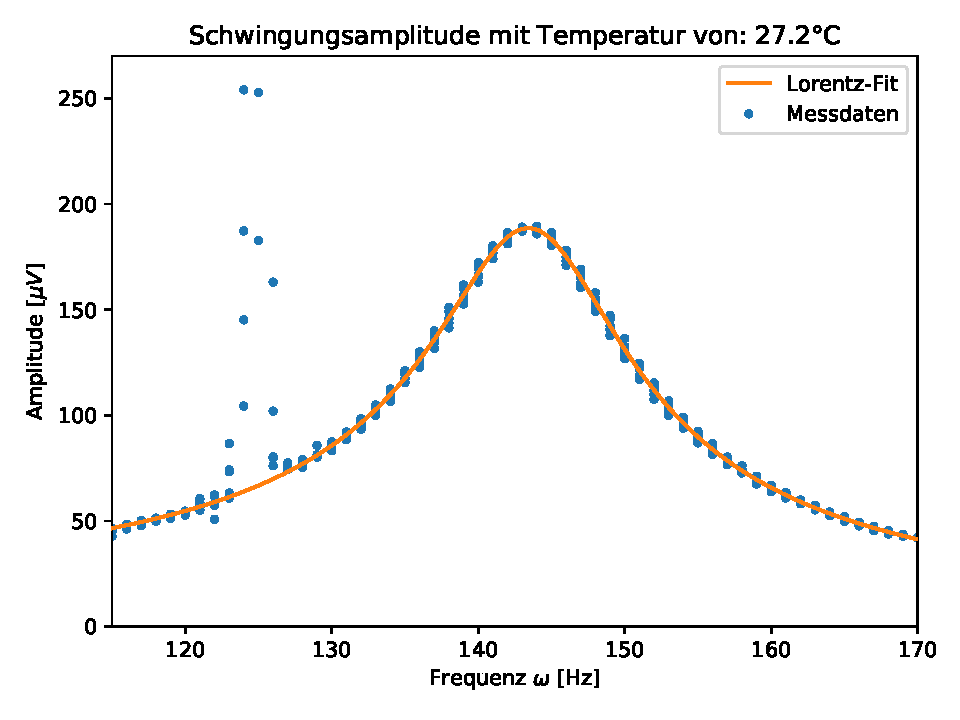
\includegraphics[width=0.5\textwidth]{Resonanz140_temp3.pdf}
\end{figure}
\begin{figure}
\centering
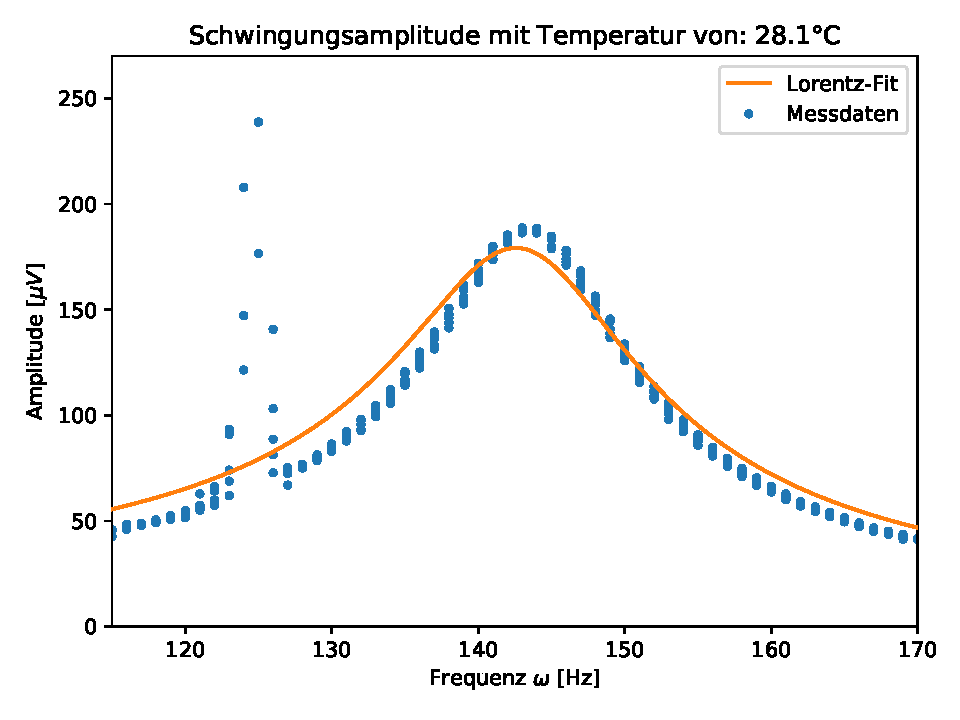
\includegraphics[width=0.5\textwidth]{Resonanz140_temp4.pdf}
\end{figure}
\begin{figure}
\centering
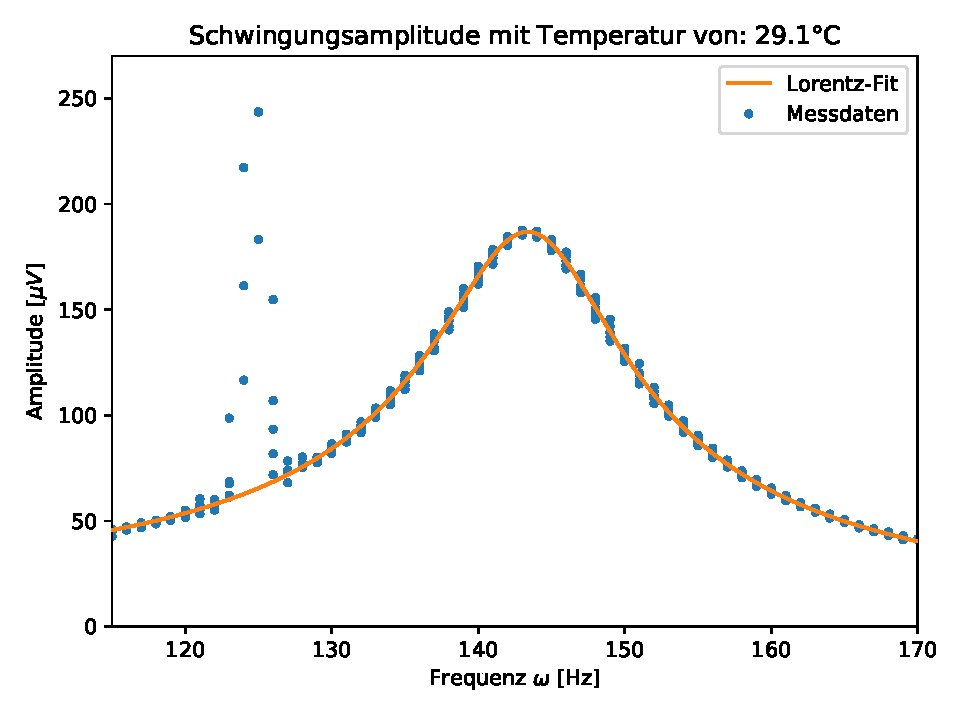
\includegraphics[width=0.5\textwidth]{Resonanz140_temp5.pdf}
\end{figure}
\begin{figure}
\centering
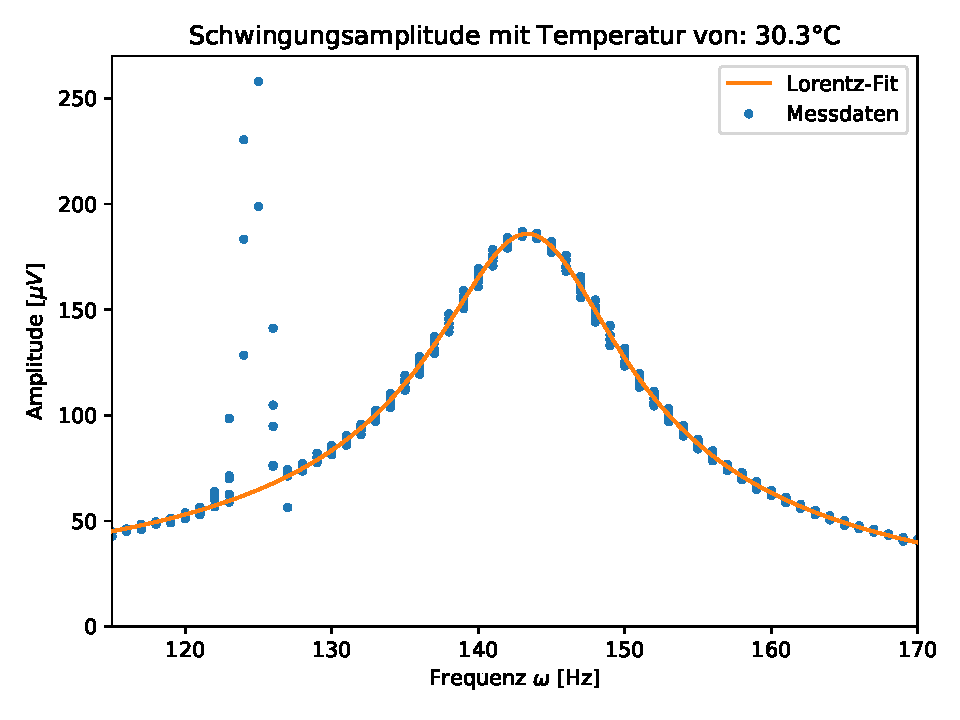
\includegraphics[width=0.5\textwidth]{Resonanz140_temp6.pdf}
\end{figure}
\begin{figure}
\centering
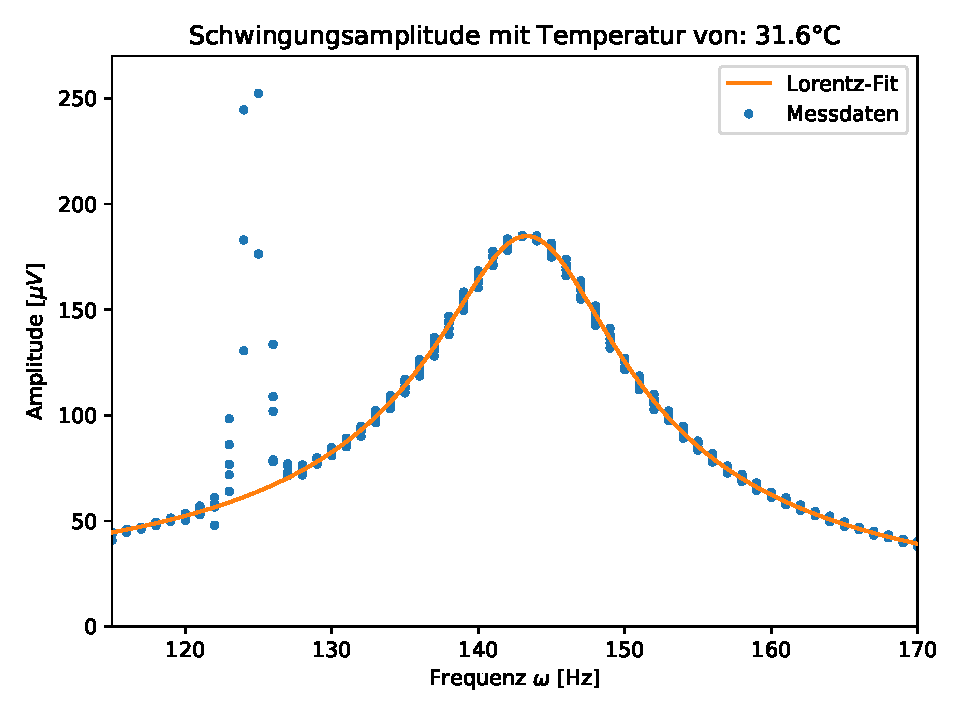
\includegraphics[width=0.5\textwidth]{Resonanz140_temp7.pdf}
\end{figure}
\begin{figure}
\centering
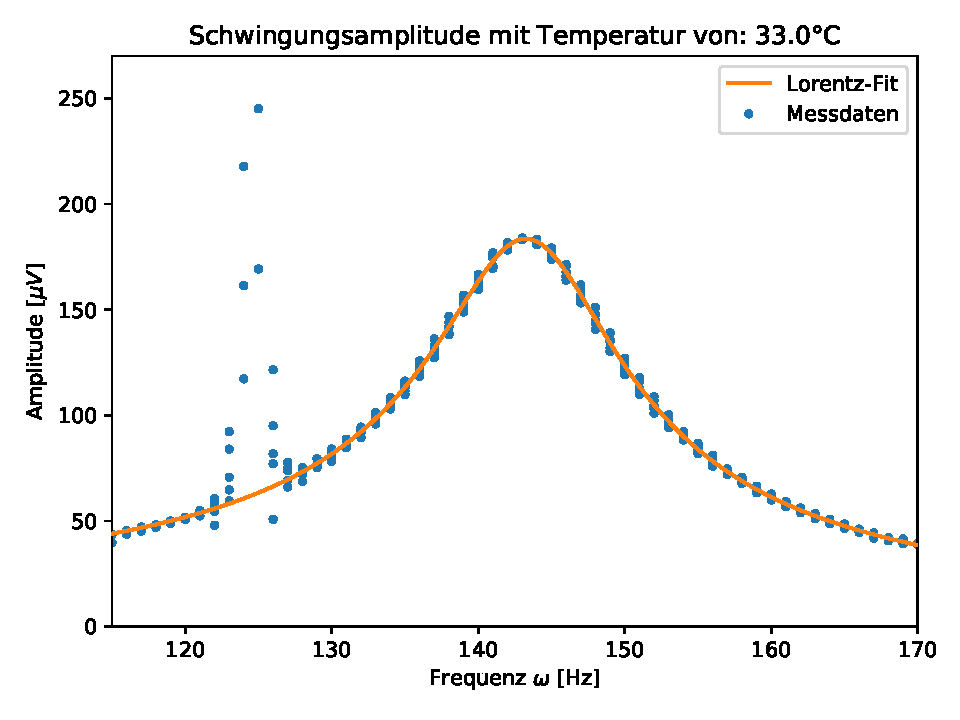
\includegraphics[width=0.5\textwidth]{Resonanz140_temp8.pdf}
\end{figure}
\begin{figure}
\centering
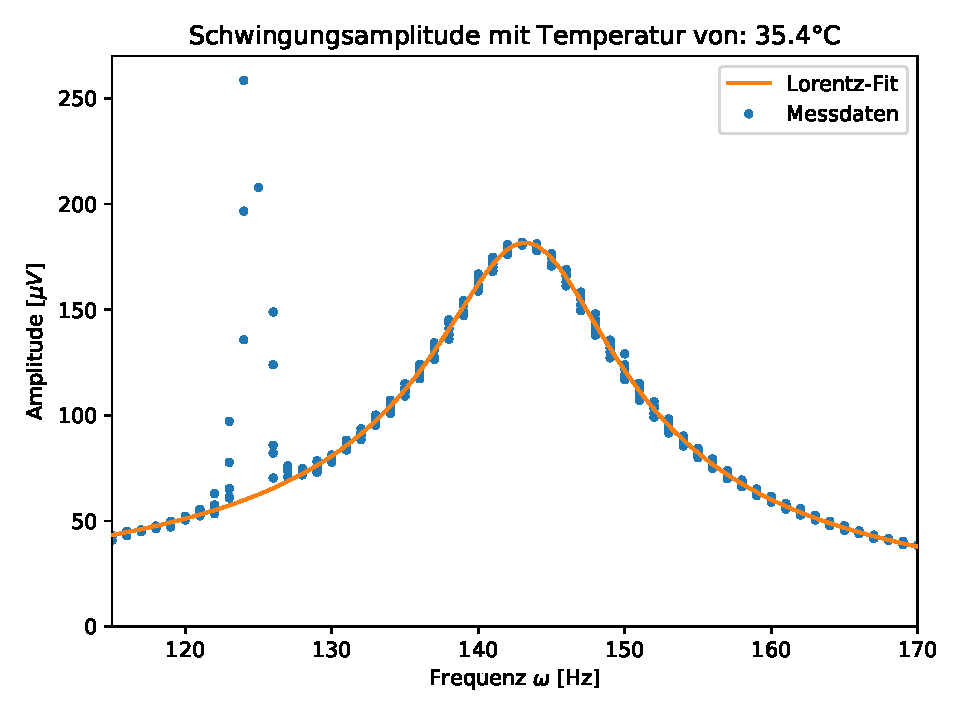
\includegraphics[width=0.5\textwidth]{Resonanz140_temp9.pdf}
\end{figure}
\begin{figure}
\centering
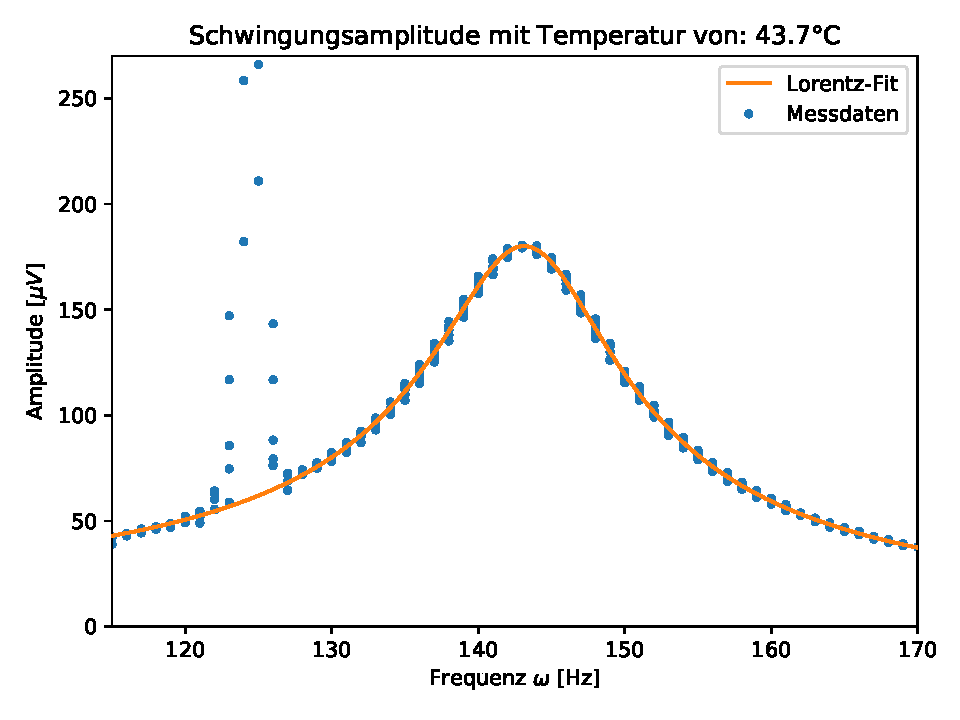
\includegraphics[width=0.5\textwidth]{Resonanz140_temp10.pdf}
\end{figure}
\begin{figure}
\centering
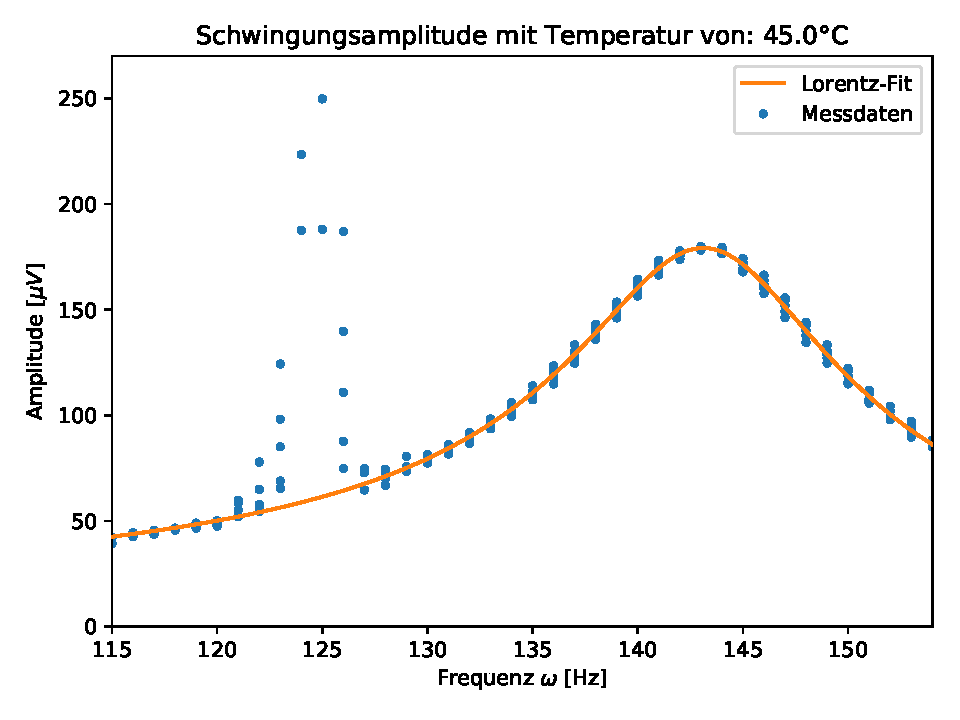
\includegraphics[width=0.5\textwidth]{Resonanz140_temp11.pdf}
\end{figure}
\end{document}